% Document Style
\documentclass[a4paper,10pt]{article}
\usepackage[left=2cm, right=2cm, top=3cm, bottom=3cm]{geometry}

% Title Page
\title{\textbf{Adjustable Support Cage for Copper Windings}}
\author{by Preston Whiteman, Maria Lytvyn-Johannesdottir, Catherine Murray, \\ Corey Firkins, Juljan Koleci, and Ahmed Wahid\and \\ \textit{City of Stoke-on-Trent Sixth Form College}}
\date{April 2024}

% References
\usepackage[backend=biber, style=phys]{biblatex}
\addbibresource{references.bib}

% Images
\usepackage{lscape}
\usepackage{rotating}
\usepackage{graphicx}
\graphicspath{{Assets/}}

% Other Packages
\usepackage{todonotes}
\usepackage{gensymb}
\usepackage{mathptmx}
\usepackage{float}
\usepackage{glossaries}

% Glossary
\makeglossaries

\newglossaryentry{WhatsApp}
{
    name=\textit{WhatsApp}
    description={WhatApp is a popular messaging application owned by Facebook. It allows users to send text messages, voice messages, images, videos, and documents, as well as make voice and video calls over the internet. We used}
}

\newglossaryentry{WddnSptCages}
{
  name=\textit{Wooden Support Cages},
  description={- \gls{GE}'s current solution which is made from wood and not adjustable}
}

\newglossaryentry{EDT}
{
  name=\textit{EDT Industrial Cadets Gold},
  description={- An industry led quality benchmark for us outreach and education programs to build pathways through education and employment}
}

\newglossaryentry{GE}
{
  name=\textit{GE Vernova Transformers},
  description={- A part of the company General Electric, operating in Stafford}
}

\newglossaryentry{gcal}{
    name={Gcal},
    description={- A shorthand term for Google Calendar, a web-based calendar service provided by Google.}
}

\newglossaryentry{reality-composer}
{
  name=\textit{Reality Composer},
  description={- An application on iPad and iPhone for developing 3D Models typically for AR}
}

\newglossaryentry{AR}
{
  name=\textit{Augmented Reality},
  description={- A way to place objects into the real world using a device's camera and screen}
}

\newglossaryentry{iPad}
{
  name=\textit{Apple iPad},
  description={- A tablet computer developed by Apple which some of us made use of during our project}
}

\newglossaryentry{CAD}
{
  name=\textit{Computer Aided Design},
  description={- The use of a computer to help and to aid the design of 2D and 3D models, interfaces, logos, etc}
}

\newglossaryentry{gantt-chart}
{
  name=\textit{Gantt Chart},
  description={- A chart created by Henry Laurence Gantt, to plan out projects at a large scale}
}

\newglossaryentry{figma}
{
  name=\textit{Figma},
  description={- An online web application for doing 2D designs}
}

\newglossaryentry{LaTeX}
{
  name=\LaTeX,
  description={- A document preparation system employed to facilitate the creation and publication of scientific documents}
}

\newglossaryentry{fischer-technik}
{
  name=\textit{Fischer Technik},
  description={- A plastic modelling set which we used to experiment with initial ideas}
}

\newglossaryentry{DMU}
{
  name=\textit{De Montford University},
  description={- A University in Leicester that kindly let us use their engineering facilities while on our residential trip}
}


\begin{document}


% ████████╗██╗████████╗██╗░░░░░███████╗  ██████╗░░█████╗░░██████╗░███████╗ %
% ╚══██╔══╝██║╚══██╔══╝██║░░░░░██╔════╝  ██╔══██╗██╔══██╗██╔════╝░██╔════╝ %
% ░░░██║░░░██║░░░██║░░░██║░░░░░█████╗░░  ██████╔╝███████║██║░░██╗░█████╗░░ %
% ░░░██║░░░██║░░░██║░░░██║░░░░░██╔══╝░░  ██╔═══╝░██╔══██║██║░░╚██╗██╔══╝░░ %
% ░░░██║░░░██║░░░██║░░░███████╗███████╗  ██║░░░░░██║░░██║╚██████╔╝███████╗ %
% ░░░╚═╝░░░╚═╝░░░╚═╝░░░╚══════╝╚══════╝  ╚═╝░░░░░╚═╝░░╚═╝░╚═════╝░╚══════╝ %

\maketitle
\begin{center}
    
\includegraphics[width = 6cm, height = 1.5cm]{logos.png}
\end{center}
\pagebreak


% ░█████╗░░█████╗░███╗░░██╗████████╗███████╗███╗░░██╗████████╗░██████╗ %
% ██╔══██╗██╔══██╗████╗░██║╚══██╔══╝██╔════╝████╗░██║╚══██╔══╝██╔════╝ %
% ██║░░╚═╝██║░░██║██╔██╗██║░░░██║░░░█████╗░░██╔██╗██║░░░██║░░░╚█████╗░ %
% ██║░░██╗██║░░██║██║╚████║░░░██║░░░██╔══╝░░██║╚████║░░░██║░░░░╚═══██╗ %
% ╚█████╔╝╚█████╔╝██║░╚███║░░░██║░░░███████╗██║░╚███║░░░██║░░░██████╔╝ %
% ░╚════╝░░╚════╝░╚═╝░░╚══╝░░░╚═╝░░░╚══════╝╚═╝░░╚══╝░░░╚═╝░░░╚═════╝░ %

\tableofcontents
\pagebreak


% ░█████╗░░█████╗░██╗░░██╗███╗░░██╗░█████╗░░██╗░░░░░░░██╗██╗░░░░░███████╗██████╗░░██████╗░███████╗███╗░░░███╗███████╗███╗░░██╗████████╗░██████╗ %
% ██╔══██╗██╔══██╗██║░██╔╝████╗░██║██╔══██╗░██║░░██╗░░██║██║░░░░░██╔════╝██╔══██╗██╔════╝░██╔════╝████╗░████║██╔════╝████╗░██║╚══██╔══╝██╔════╝ %
% ███████║██║░░╚═╝█████═╝░██╔██╗██║██║░░██║░╚██╗████╗██╔╝██║░░░░░█████╗░░██║░░██║██║░░██╗░█████╗░░██╔████╔██║█████╗░░██╔██╗██║░░░██║░░░╚█████╗░ %
% ██╔══██║██║░░██╗██╔═██╗░██║╚████║██║░░██║░░████╔═████║░██║░░░░░██╔══╝░░██║░░██║██║░░╚██╗██╔══╝░░██║╚██╔╝██║██╔══╝░░██║╚████║░░░██║░░░░╚═══██╗ %
% ██║░░██║╚█████╔╝██║░╚██╗██║░╚███║╚█████╔╝░░╚██╔╝░╚██╔╝░███████╗███████╗██████╔╝╚██████╔╝███████╗██║░╚═╝░██║███████╗██║░╚███║░░░██║░░░██████╔╝ %
% ╚═╝░░╚═╝░╚════╝░╚═╝░░╚═╝╚═╝░░╚══╝░╚════╝░░░░╚═╝░░░╚═╝░░╚══════╝╚══════╝╚═════╝░░╚═════╝░╚══════╝╚═╝░░░░░╚═╝╚══════╝╚═╝░░╚══╝░░░╚═╝░░░╚═════╝░ %

\section{Acknowledgments}
\subsection{Ourselves}
We all contributed to the project, notably:
\begin{itemize}
  \item{\textit{Preston Whiteman} - Team leader, organiser and head report writer}
    \subitem{Wrote most of and collected the report into a \gls{LaTeX} document, designed solutions and came up with ideas, coordinated team members so that they could work together. Also planned out most of the project and designed almost all 3D \gls{CAD} models}
  \item{\textit{Maria Lytvyn-Johannesdottir} - Head note taker, Writing}
    \subitem{Took photos while at \gls{GE} and was the head note taker for our team. Came up with many ideas and contributed to others. Wrote Ideas chapter.}
  \item{\textit{Catherine Murray} - Writing, Building and Design}
    \subitem{Wrote the Introduction chapter, contributed heavily to ideas and design. When on residential trip in Leicester helped to create final prototype.}
  \item{\textit{Corey Firkins} - Writing, Building and Design}
    \subitem{Made the cardboard model and contributed to efforts of making the final prototype. Wrote up the Leicester trip visit and cardboard model sections of the report.}
  \item{\textit{Juljan Koleci} }
  \item{\textit{Ahmed Wahid} - Ideas and Building}
    \subitem{Helped to contribute to ideas and came up with the Adjustable Sliding Mechanism idea. When in Leicester helped to assemble the final model prototype.}
\end{itemize}

\subsection{Others}
We express our gratitude to the following individuals and organisations:
\begin{itemize}
  \item{\textit{David Sellers} - For coordinating the project, providing continuous guidance, and being readily available to address any inquiries related to the project, ensuring our progress was on course.}
  \item{\textit{Mick Stevens} - For offering guidance, representing \gls{GE}, and assisting us with any questions pertaining to the problem and \gls{GE} as required.}
  \item{\textit{EDT Industrial Cadets}}
  \item{\gls{GE}}
  \item {\gls{DMU}}
\end{itemize}
\pagebreak


% ██╗███╗░░██╗████████╗██████╗░░█████╗░██████╗░██╗░░░██╗░█████╗░████████╗██╗░█████╗░███╗░░██╗ %
% ██║████╗░██║╚══██╔══╝██╔══██╗██╔══██╗██╔══██╗██║░░░██║██╔══██╗╚══██╔══╝██║██╔══██╗████╗░██║ %
% ██║██╔██╗██║░░░██║░░░██████╔╝██║░░██║██║░░██║██║░░░██║██║░░╚═╝░░░██║░░░██║██║░░██║██╔██╗██║ %
% ██║██║╚████║░░░██║░░░██╔══██╗██║░░██║██║░░██║██║░░░██║██║░░██╗░░░██║░░░██║██║░░██║██║╚████║ %
% ██║██║░╚███║░░░██║░░░██║░░██║╚█████╔╝██████╔╝╚██████╔╝╚█████╔╝░░░██║░░░██║╚█████╔╝██║░╚███║ %
% ╚═╝╚═╝░░╚══╝░░░╚═╝░░░╚═╝░░╚═╝░╚════╝░╚═════╝░░╚═════╝░░╚════╝░░░░╚═╝░░░╚═╝░╚════╝░╚═╝░░╚══╝ %

\section{Introduction}
This report documents our accomplished results in the creation of an Adjustable Support Cage for Copper Windings designed for \gls{GE}. It serves as a comprehensive documentation of our research, design, and development process. It is important to note that this project was undertaken as part of the \gls{EDT} Award.

\subsection{GE Vernova}
\begin{figure}[H]
  \centering
  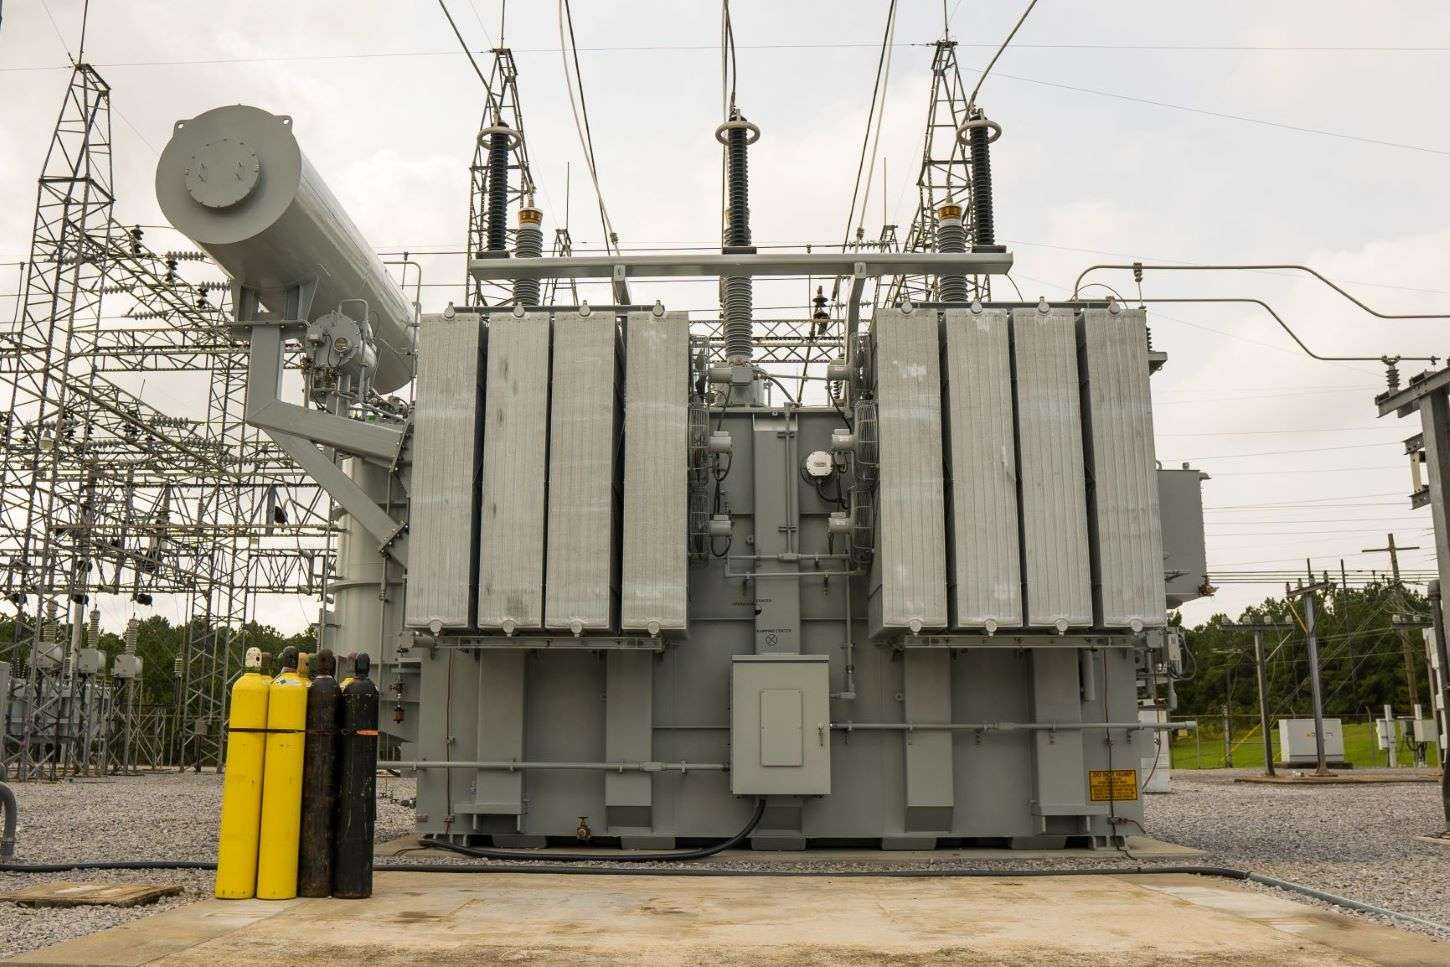
\includegraphics[width=6cm]{giant-transformer}
  \caption{A giant transformer produced by \gls{GE}}
  \label{fig:giant-transformer}
\end{figure}

\gls{GE} is a division of General Electric, operating in Stafford, specializing in the construction of massive transformers predominantly used in high voltage power grids. Our visit to \gls{GE} on November 21, 2023, proved invaluable as we gained insights into the project. The guided tour showcased the \gls{WddnSptCages}, and the company's explanations provided a solid foundation for our project goals.

\subsection{The Cages}
\begin{figure}[H]
  \centering
  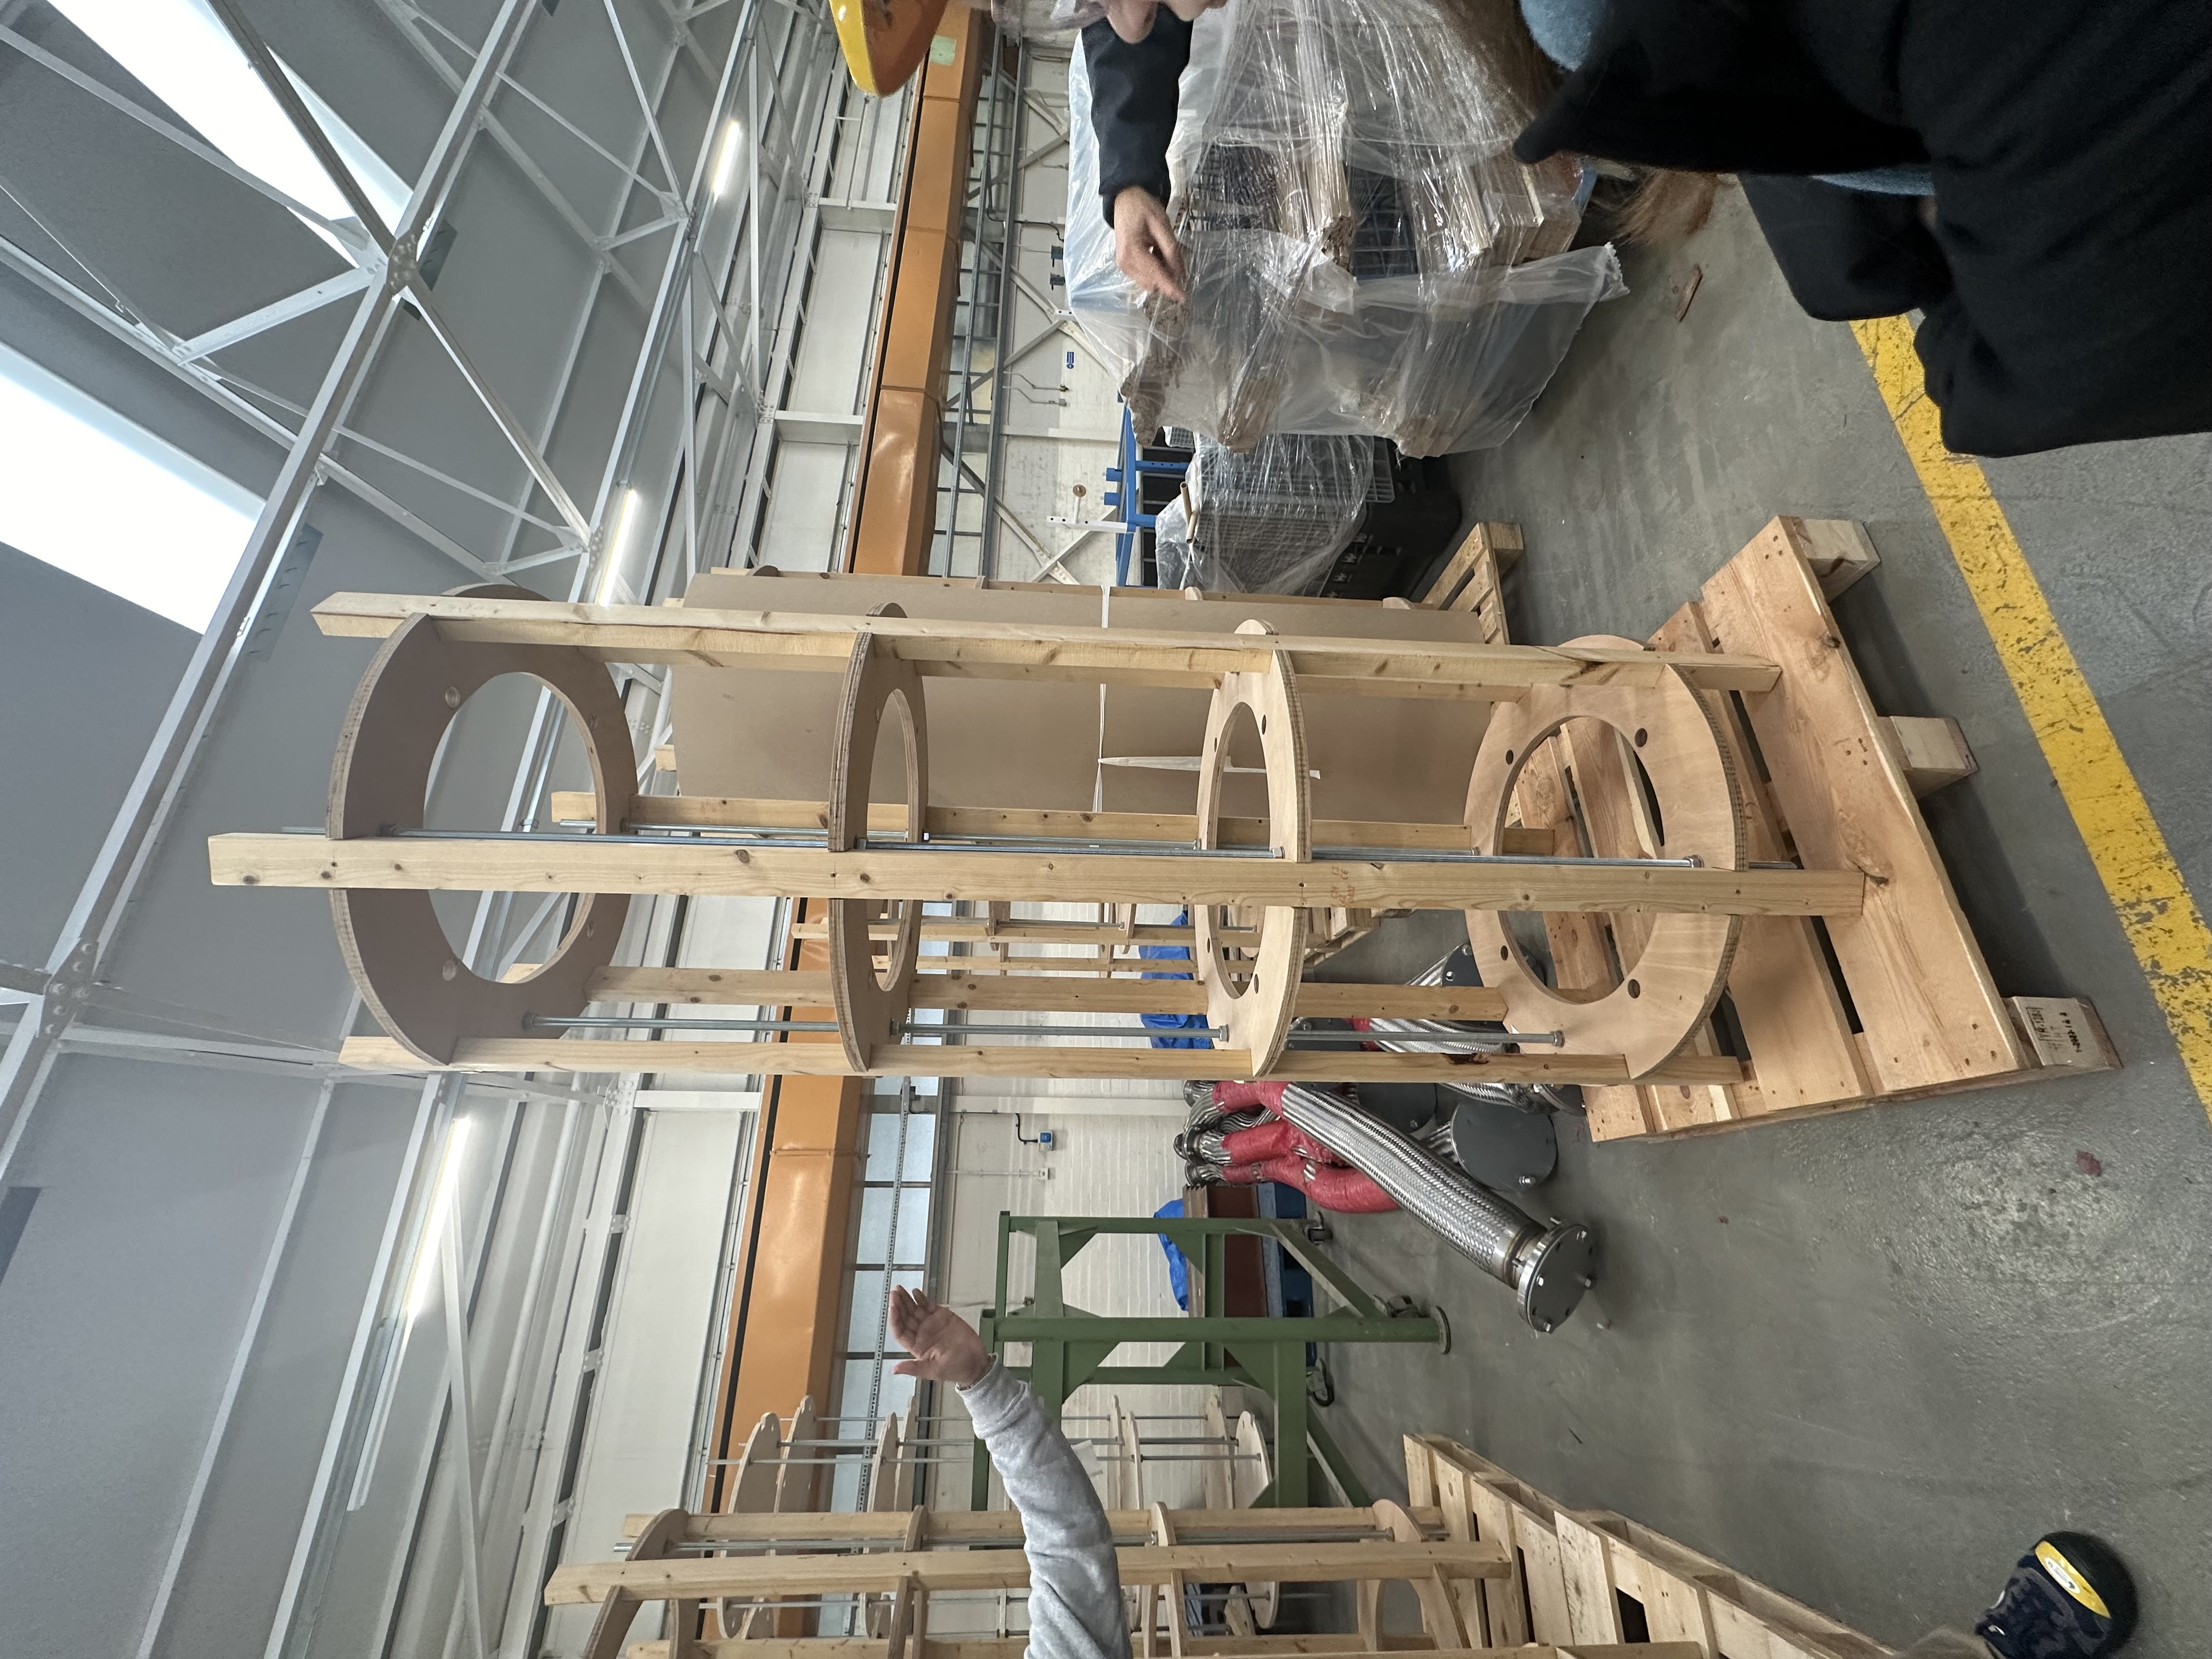
\includegraphics[width=6cm, angle=270]{wooden-support-cage}
  \caption{\gls{WddnSptCages}}
  \label{fig:wooden-support-cage}
\end{figure}

We also explored the procedure for how \gls{GE} utilises the support cages within their manufacturing process.

\subsection{The Problem}
The STEM Project for 2024 focuses on designing an Adjustable Support Cage for windings. During the winding manufacture process, coils are wound on vertical or horizontal lathes and then clamped under mechanical pressure for oven drying. In windings with a small radial depth, support cages are inserted to enhance mechanical stability, preventing collapse under heat and pressure.

Currently, these support cages are customised for specific windings, with limited adjustability achieved by exchanging outer battens. Our project aims to review and redesign these cages for greater adjustability.

\subsection{Project Objectives}
\begin{itemize}
  \item Review data on expected winding diameters (provided by \gls{GE}).
  \item Examine existing non-adjustable support cages.
  \item Investigate the available adjustability methods.
  \item Define a method and range of adjustment achievable.
\end{itemize}

\subsection{Expected Benefits}
\begin{itemize}
  \item Reduction in material cost for each winding.
  \item Decrease in engineering hours for \gls{GE}.
  \item Simplification in the production process.
\end{itemize}

The existing cages are currently tailor-made to specific winding requirements, emphasising the need for a more adjustable solution.


% ████████╗███████╗░█████╗░███╗░░░███╗░░░░░░░██╗░░░░░░░██╗░█████╗░██████╗░██╗░░██╗██╗███╗░░██╗░██████╗░ %
% ╚══██╔══╝██╔════╝██╔══██╗████╗░████║░░░░░░░██║░░██╗░░██║██╔══██╗██╔══██╗██║░██╔╝██║████╗░██║██╔════╝░ %
% ░░░██║░░░█████╗░░███████║██╔████╔██║█████╗░╚██╗████╗██╔╝██║░░██║██████╔╝█████═╝░██║██╔██╗██║██║░░██╗░ %
% ░░░██║░░░██╔══╝░░██╔══██║██║╚██╔╝██║╚════╝░░████╔═████║░██║░░██║██╔══██╗██╔═██╗░██║██║╚████║██║░░╚██╗ %
% ░░░██║░░░███████╗██║░░██║██║░╚═╝░██║░░░░░░░░╚██╔╝░╚██╔╝░╚█████╔╝██║░░██║██║░╚██╗██║██║░╚███║╚██████╔╝ %
% ░░░╚═╝░░░╚══════╝╚═╝░░╚═╝╚═╝░░░░░╚═╝░░░░░░░░░╚═╝░░░╚═╝░░░╚════╝░╚═╝░░╚═╝╚═╝░░╚═╝╚═╝╚═╝░░╚══╝░╚═════╝░ %

\section{Team working}
In our project aimed at designing a model of an adjustable birdcage for the transformer, effective communication played a pivotal role in ensuring the success of our endeavor. Here's how we utilized various tools and methods to facilitate seamless collaboration within our team:

\subsection{Shared Gcal}
We leveraged a shared Google calendar to coordinate our schedules and find overlapping free time slots. This allowed us to efficiently allocate dedicated time for project work, ensuring that all team members could contribute effectively without conflicting commitments.

\subsection{Shared Gdocs}
Utilising Google Docs enabled us to collaborate on the project report in real-time. With this platform, multiple team members could work on the same document simultaneously, facilitating efficient brainstorming, editing, and feedback exchange.

\subsection{Shared Gdrive}
The use of a shared Google Drive served as a centralized repository for all project-related files and resources. This streamlined collaboration by providing a convenient platform for storing, organizing, and accessing documents, data, and other project materials collectively.

\subsection{WhatsApp Group Chat}
 In addition to scheduled meetings, we maintained a dedicated WhatsApp group for informal communication and quick exchanges outside of formal meetings. This platform facilitated swift information sharing, idea generation, and clarification of doubts or queries, promoting ongoing engagement and collaboration among team members.

\subsection{Weekly team meetings}
We conducted regular face-to-face team meetings on a weekly basis. These meetings served as valuable opportunities to discuss project progress, brainstorm ideas, allocate tasks, and prepare for upcoming milestones. Additionally, these sessions allowed us to refine our project approach, troubleshoot challenges, and rehearse our presentation skills.


% ██╗██████╗░███████╗░█████╗░░██████╗ %
% ██║██╔══██╗██╔════╝██╔══██╗██╔════╝ %
% ██║██║░░██║█████╗░░███████║╚█████╗░ %
% ██║██║░░██║██╔══╝░░██╔══██║░╚═══██╗ %
% ██║██████╔╝███████╗██║░░██║██████╔╝ %
% ╚═╝╚═════╝░╚══════╝╚═╝░░╚═╝╚═════╝░ %


\section{Ideas}
Once we had received information about our prompt, we immediately began to write down and draw up any potential solutions. After much contemplating and the site visit for more information, we narrowed it down to one solution. The ideas are listed in chronological order.

\subsection{Geometric Expanding Table}

\subsubsection{description}

Once I understood that the contraption must be adjustable, my first thought was an expanding geometric table. It can expand from a small set diameter to a larger set diameter by adding more pieces. We thought if this concept could translate to our holding cages.

\begin{figure}[H]
  \centering
  \includegraphics[width=15cm]{Assets/adjustable-block-notes.png}
  \caption{Notes to demonstrate the functionality of the Adjustable Sliding Mechanism}
  \label{fig:adjustable-block-notes}
\end{figure}

\subsubsection{Strengths and Weaknesses}

\begin{table}[h]
  \centering
  \begin{tabular}{p{0.5\linewidth} | p{0.5\linewidth}}
    Strengths                                              & Weaknesses \\ \hline
    \textbullet{} Can be adjusted                          & \textbullet{} Only set to two diameters when a range is required \\
    \textbullet{} Specifically circular                    & \textbullet{} Unsure how it would work vertically \\
    \textbullet{} Simple mechanism                         & \textbullet{} Too complicated mechanically \\
  \end{tabular}
  \caption{Strengths and Weaknesses of the Geometric Expanding Table}
  \label{table:geometric-expanding-table-pros-cons}
\end{table}

\subsection{Adjustable Sliding Mechanism}

\subsubsection{Description}

This idea proposes the creation of a rectangular metal block with strategically placed holes to accommodate various measurements required in transformer winding support. This block is designed to slide into a hollow sleeve, offering a dynamic and adjustable support mechanism. The idea aims to strike a balance between simplicity and versatility, allowing the support block to accommodate different winding diameters.

\begin{figure}[H]
  \centering
  \includegraphics[width=15cm]{Assets/adjustable-block-notes.png}
  \caption{Notes to demonstrate the functionality of the Adjustable Sliding Mechanism}
  \label{fig:adjustable-block-notes}
\end{figure}

\subsubsection{Strengths and Weaknesses}

\begin{table}[h]
  \centering
  \begin{tabular}{p{0.5\linewidth} | p{0.5\linewidth}}
    Strengths                                              & Weaknesses \\ \hline
    \textbullet{} Pretty straightforward                   & \textbullet{} Not variable enough for certain measurements \\
    \textbullet{} Easy to adjust                           & \textbullet{} Trade-off with rigidity when increasing variability \\
    \textbullet{} Fairly rigid structure                   & \textbullet{} Too much effort to adjust every bolt \\
  \end{tabular}
  \caption{Strengths and Weaknesses of the Adjustable Sliding Mechanism}
  \label{table:adjustable-block-pros-cons}
\end{table}

\section{}


\pagebreak
\printglossaries

\end{document}